\subsubsection{Hash table}
\label{sec:hash}

\usetikzlibrary{shapes.multipart,positioning,arrows,calc}
\tikzset{
  listnode/.style={
    rectangle split,rectangle split parts=2,draw,rectangle split horizontal,fill=blue!20
  },
  startnode/.style={
    draw,minimum width=1.5cm,minimum height=.75cm
  }
}

\begin{figure}
  \centering
  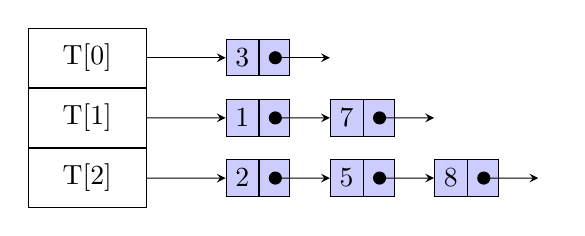
\begin{tikzpicture}[scale=.2, >=stealth]
    \node[startnode] (t0) {T[0]};
    \node[startnode,below=0pt of t0] (t1) {T[1]};
    \node[startnode,below=0pt of t1] (t2) {T[2]};
    \node[listnode,right=of t0] (3) {3};
    \node[listnode,right=of t1] (1) {1};
    \node[listnode,right=.5cm of 1] (7) {7};
    \node[listnode,right=of t2] (2) {2};
    \node[listnode,right=.5cm of 2] (5) {5};
    \node[listnode,right=.5cm of 5] (8) {8};
    \node[right=.5cm of 3] (3x) {$\varnothing$};
    \node[right=.5cm of 7] (7x) {$\varnothing$};
    \node[right=.5cm of 8] (8x) {$\varnothing$};
    \draw[*->] let \p1 = (3.two), \p2 = (3.center) in (\x1,\y2) -- (3x);
    \draw[*->] let \p1 = (1.two), \p2 = (1.center) in (\x1,\y2) -- (7);
    \draw[*->] let \p1 = (7.two), \p2 = (7.center) in (\x1,\y2) -- (7x);
    \draw[*->] let \p1 = (2.two), \p2 = (2.center) in (\x1,\y2) -- (5);
    \draw[*->] let \p1 = (5.two), \p2 = (5.center) in (\x1,\y2) -- (8);
    \draw[*->] let \p1 = (8.two), \p2 = (8.center) in (\x1,\y2) -- (8x);
    \draw[->] (t0) edge (3) (t1) edge (1) (t2) edge (2);
  \end{tikzpicture}

  \caption{Representação da tabela \textit{hash} com três \textit{buckets}
    implementados utilizando listas ligadas.}
  \label{fig:hash}
\end{figure}